\chapter{Query Builder}
\label{chapter:QB}

This project has another goal: to enhance the conversational search assistant to collect additional information in order to provide a query as an outcome. The query is referred to as cohort definition in the ATLAS community, as detailed in section \ref{atlas}.

The following section discusses the implementation of the query builder, as well as the decisions and strategies involved.


\section{Implementation Strategy}

% explicar a estratégia de implementação do query builder
%   criação de 2 ficheiros: o cohort template e outro com as respetivas perguntas para cada field
%   pointer para o campo a ser analisado
%   divisão do query builder em 2 partes: concept set and cohort definition

To create a system that builds a query through a conversation with the user, the first step is to get a cohort definition generated in the ATLAS platform after implementing an experimental case. Understanding how the cohort is built is crucial at this stage. The section \ref{atlas} details defining a cohort. The definition of a cohort requires the definition of a concept set. So, the strategy of the cohort construction is focused first on creating the concept set and then on the rest of the cohort's parameters.


\subsection{Interaction between Components}

It is important to understand how this system interacts with the user and other external tools. Diagram \ref{fig_interaction} describes all the interactions between components. The interaction diagram all the interactions between components. The system components are the {\ir} API and the Chatbot Interface, which contains the User interface and the {\llm}. The {\ehden} Portal and ATLAS are external tools.

\begin{figure}[H]
  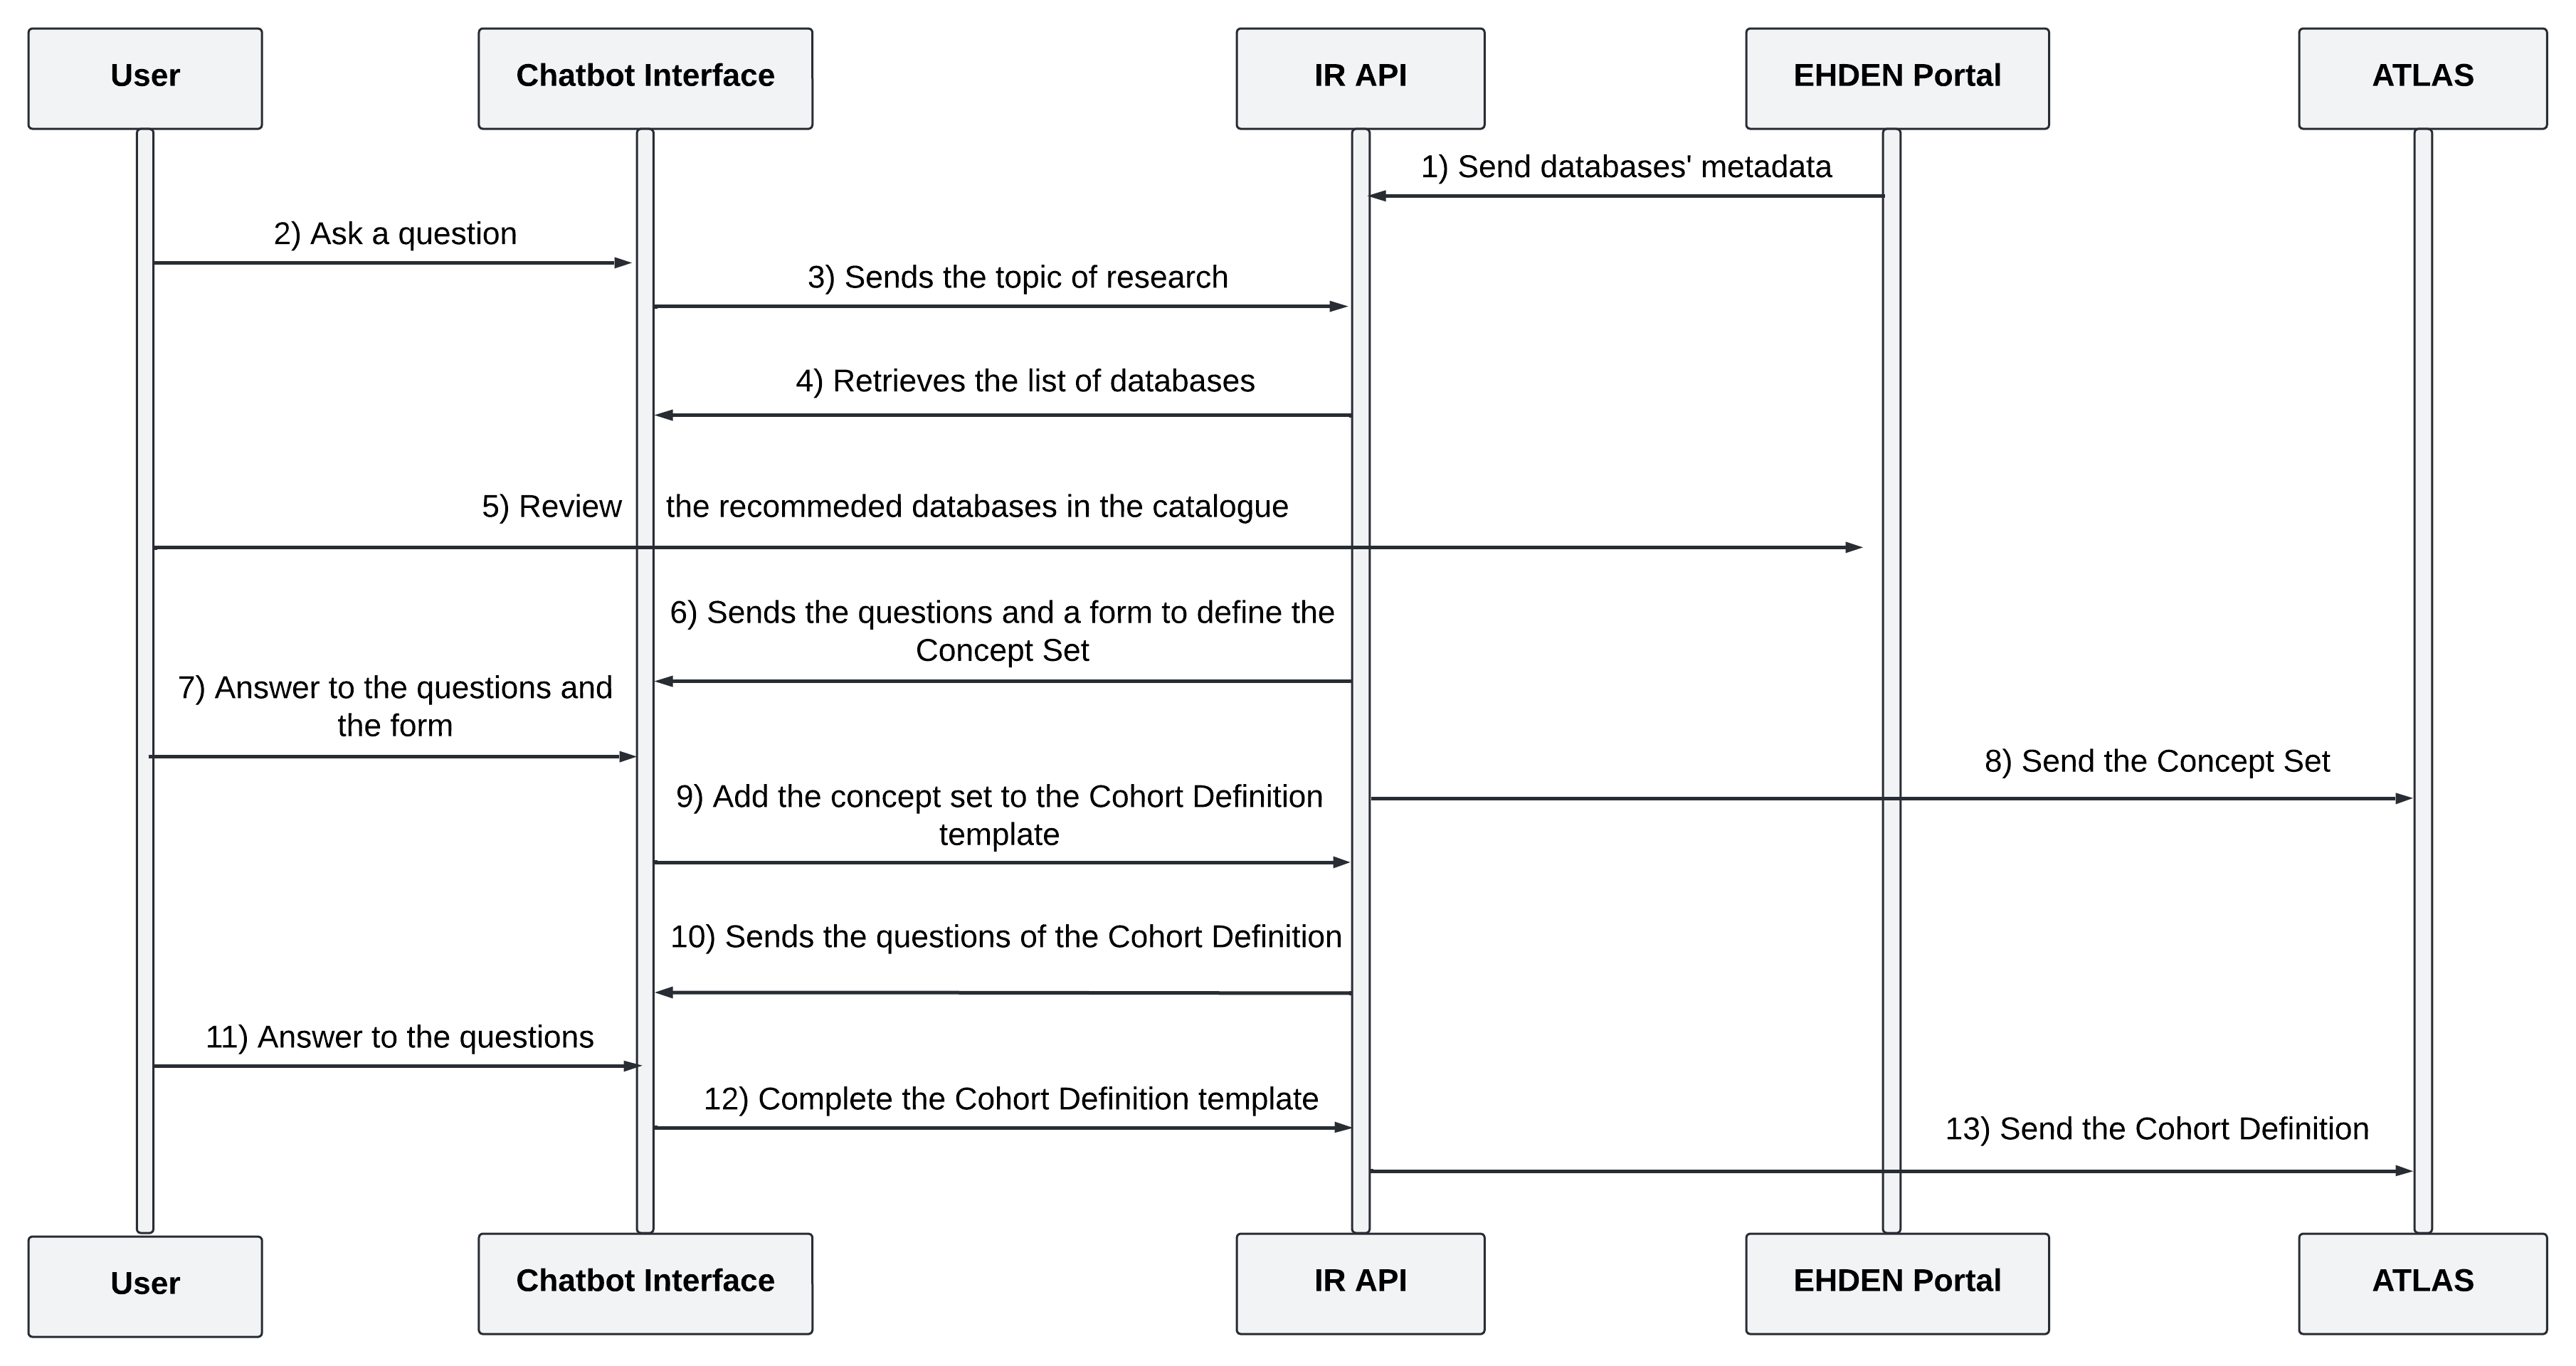
\includegraphics[width=\textwidth]{figs/chapter4/interaction_diagram1.png}
  \centering
  \caption{Interaction diagram between the user, the system components and external tools.}
  \label{fig_interaction}
\end{figure}

This diagram presents all the interactions of the conversational query builder, not only presenting the interactions detailed in the previous chapter \ref{chapter:ConversationalSearchAssistant} — steps 1) to 5) —, but also the interactions that will be performed during the detail of this chapter — steps 6) to 13).

Reminding the interactions explained in chapter \ref{chapter:ConversationalSearchAssistant}, the {\ir} component receives the databases' metadata from the {\ehden} Portal — step 1) —, creating and indexing the documents. The user asks a question to the Chatbot Interface — step 2). Here, the {\llm} applies his task of identifying the research topic and sends it to the {\ir} API — step 3). The {\ir} API retrieves the most suitable databases for the research concept and sends the list of databases to the Chatbot Interface — step 4). The user can review the recommended databases in the catalogue in the {\ehden} Portal — step 5). 

Now, the query builder phase starts. As mentioned before, the cohort's construction requires a concept set. So, the {\ir} API, when sending the databases to the chatbot interface, also sends questions and then a form to help define the concept set — step 6). The user answers the question and fills out the form — step 7 —, in order to create the Concept Set that could be sent to the ATLAS instance — step 8). 

The rest of the cohort will be determined now that the concept set is defined. The Concept Set is added to the cohort definition template  — step 9). The {\ir} API sends a question to complete a field needed for the cohort definition  — step 10). After the user answers to it  — step 11) —, the {\llm}, in the Chatbot Interface, analyses if the user message is an answer to the question. If so, the answer will be saved in the cohort template — step 12). Steps 10), 11), and 12) are repeated until the cohort template is complete. Finally, the {\ir} API sends the cohort definition to the ATLAS instance if the user requests it — step 13).


\subsection{Template and Questions}

The ATLAS platform accepts the import of a cohort definition in a JSON format. Two crucial JSON files are needed to generate this JSON object, personalized with the user's requirements information. One is the template for users to fill out during the conversation {\small\normalfont(\texttt{cohort\_template.json})}, shown in Code \ref{template}. This template is an empty cohort definition JSON structure. The other file, Code \ref{questions}, is the questions associated with each key field of the template {\small\normalfont(\texttt{cohort\_questions.json})}. Each question should be simple and efficient so the medical researcher can respond to it, and its response is the value of that key. Also, each question in the template is manually inserted in the JSON file.  

\begin{listing}[H]
  \begin{minted}[breaklines]{json}
      
    {
      "ConceptSets": null,
      "PrimaryCriteria": {
          "CriteriaList": [
              {
                  "ConditionOccurrence": {
                      "CodesetId": 0,
                      "ConditionTypeExclude": null,
                      "ConditionSourceConcept": null,
                      "First": null
                  }
              }
          ],
          "ObservationWindow": {
              "PriorDays": 0,
              "PostDays": 0
          },
          "PrimaryCriteriaLimit": {
              "Type": "First"
          }
      },
      "QualifiedLimit": {
          "Type": "First"
      },
      "ExpressionLimit": {
          "Type": "First"
      },
      "InclusionRules": [],
      "CensoringCriteria": [],
      "CollapseSettings": {
          "CollapseType": "ERA",
          "EraPad": 0
      },
      "CensorWindow": {}
  }

  \end{minted}
\caption{The cohort template file {\small\normalfont(\texttt{cohort\_template.json})}.}
\label{template}
\end{listing}  

\begin{listing}[H]
  \begin{minted}[breaklines]{json}
      
    {
      "ConceptSets": "Are there any other concepts you'd like to add? If yes, please add them. If no, simply respond with 'no'.",
    
      "PrimaryCriteria": {
        "ObservationWindow": {
          "PriorDays": "Regarding the observation window, what is the minimum number of days needed before the continuous observation? You must choose from 0, 1, 7, 14, 21, 30, 60, 90, 120, 180, 365, 548, 730 or 1095.",
          "PostDays": "How many days after event index date? You must choose from 0, 1, 7, 14, 21, 30, 60, 90, 120, 180, 365, 548, 730 or 1095."
        }
      }
    }

  \end{minted}
  \caption{The cohort questions file {\small\normalfont(\texttt{cohort\_questions.json})}.}
  \label{questions}
\end{listing}



\subsection{Template Pointer}

In a nutshell, the cohort questions file have the questions to complete the cohort template file. However, when exchanging messages with the user, tracking which questions must be asked and which question the user responded to is essential and also a problem.

The solution to this issue is creating a pointer to a template key. The pointer retrieves a template key that should be completed with the user information. The pointer points to the same key until the user responds to the question associated with the pointer. Otherwise, it moves to the following template key.

So, during the conversation, the pointer helps:

\begin{itemize}
  \item To determine the appropriate question to ask the user.
  \item To identify which key of the cohort template to use to save the user's answer.
  \item To move on to the next question of the cohort template.
\end{itemize}

This solution keeps track of the user's responses and dynamically updates the template with the relevant information throughout the conversation.


\section{Concepts Sets}

% https://ohdsi.github.io/TheBookOfOhdsi/Cohorts.html#conceptSets

In Code \ref{template}, a cohort is defined by multiple JSON fields. One of these fields is the concepts set (the cohort template key is '\textit{ConceptSets}'), which is a list of concepts required to meet the study requirements of the researcher. In order to properly define a cohort, the concept set must be established first. 

A concept set consists of standardized medical terms that define clinical elements like diseases, drugs, and procedures. Therefore, our strategy is to define the concept set in the conversation before moving on to the remaining fields of the cohort template.

This section details the creation of the concept set needed for the cohort definition later.


\subsection{Expression}
A concept set expression is comprised of a list of concepts with the following attributes:

\begin{itemize}
  \item \textbf{concept}: Definition of a concept, using data contained in the concepts file  {\small\normalfont(\texttt{concepts.csv})} (section \ref{data}).
  \item \textbf{isExcluded}: Exclude the concept from the concept set.
  \item \textbf{includeDescendants}: Add all of descendants of a concept, with it also included.
  \item \textbf{includeMapped}: Allow the search for non-standard concepts.
\end{itemize}


The JSON code \ref{conceptset} below represents a concept definition within a concept set expression. This example is not real information; it is just to define a concept set visually.

\begin{listing}[H]
  \begin{minted}[breaklines]{json}
      
    {
      "id": 0,
      "name": "<CONCEPT SET NAME>",
      "expression": {
          "items": [
              {
                  "concept": {
                      "CONCEPT_ID": 231256,
                      "CONCEPT_NAME": "Covid-19",
                      "DOMAIN_ID": "Condition",
                      "VOCABULARY_ID": "ASG67HR",
                      "CONCEPT_CLASS_ID": "ASG67 code",
                      "CONCEPT_CODE": "953635",
                      "VALID_START_DATE": "2000-01-01",
                      "VALID_END_DATE": "2099-12-31"
                  },
                  "isExcluded": false,
                  "includeDescendants": true,
                  "includeMapped": false
              },
              
              (...)
          ]
      }
    }

  \end{minted}
\caption{A Concept Set expression example.}
\label{conceptset}
\end{listing}  



\subsection{Implementation}


% 0) o utilizador insere uma query, o chatbot pergunta se ele tem mais conceitos, se sim, que os indique, até ao utilizador dizer que não tem mais conceitos para adicionar
% 1) utilizar IR para encontrar os conceitos associados à query que o user inseriu
% 2) ir buscar as informações adicionais aos ficheiro de conceitos
% 3) enviar a lista de conceitos ao utilizador e apresentar como forms 
% 4) utilizador escolhe os conceitos que quer inserir e escolhe os atributos
% 5) submete o forms, e a concept set é criado


The goal is to create a JSON object identical to the one in the Code \ref{conceptset} with the concepts selected by the medical researcher.

When a user enters a query, the conversational search assistant retrieves the best databases related to the health topic of that query. It should also inquire whether the user has additional concepts for their study requirements. In an implementation vision, the first key to complete in the cohort template is '\textit{ConceptsSets}', so the question regarding that key is rewritten by the {\llm} and then asked to the user.

The user should respond to whether there are additional concepts to add. If there are, he should indicate them. If not, he should provide a negative answer. The chatbot will continue to ask if there are more concepts until the user confirms that there are no more to add.

Now, in the {\ir} component, the {\bm} technique searches in the collection for the concepts the user indicates in his responses. After identifying each concept in the collection using the {\ir} technique search, additional information from the concept file is added. This includes the concept ID, concept code, and other attributes that define the concept as represented in Code \ref{conceptset}.

The list of concepts identified is sent to the chatbot interface. The chatbot interface shows the concepts in a form. For example, Figure \ref{fig_forms} shows a form to create the concept set after the user mentions his interest in COVID-19. The user gives a name to the concept set and selects the concepts and the other attributes.


\begin{figure}[H]
  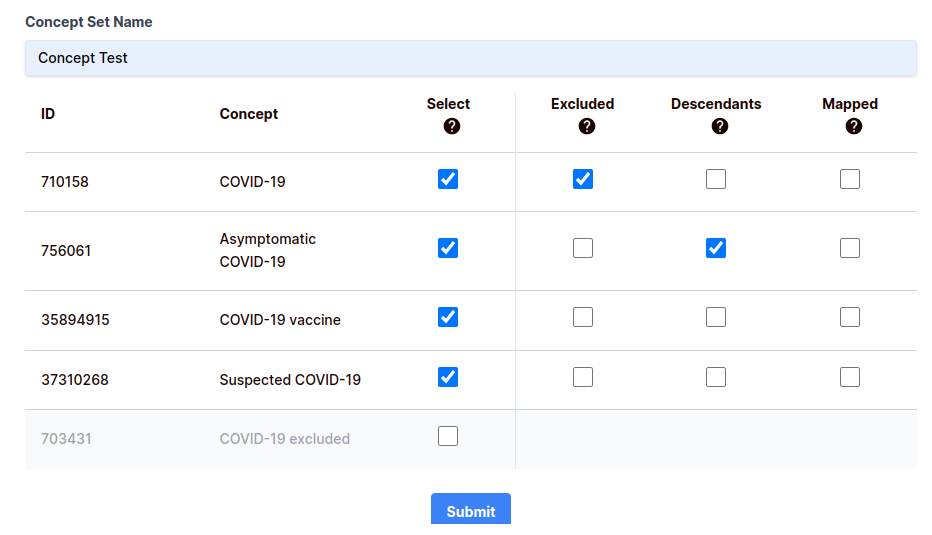
\includegraphics[width=1\textwidth]{figs/chapter4/form.png}
  \centering
  \caption{The form to create the Concept Set.}
  \label{fig_forms}
\end{figure}


Finally, the user submits the forms, creating the concept set. The chatbot will send a message informing the user that they can download the concept set JSON file, which is accepted in the ATLAS instance, to create a new concept set. Alternatively, the chatbot can send the file directly to the ATLAS instance. The pointer of the cohort template moves to the next key.



\section{Cohort Definition}

% depois do concept set estar definido, o template pointer passa para a proxima key com pergunta
% o LLM gera a pergunta e a interface apresenta-a ao utilizador
% o utilizador responde 
% o LLM verifica se a mensagem do utilizador é em resposta à pergunta
%   - se sim, atualiza o template com a resposta, e o template pointer avança
%   - se não, volta a questionar a mesma questão ao utilzador
% este ciclo repete-se até o cohort estar completo


% TODO: intro, e fazer refenciar o template

Once the Concept Set is defined, the list of concepts and their attributes are saved on the template, where the template key points to. Then, the template pointer moves to the next template key. The {\llm} generates a specific question related to the question that the current key points to. This generated question is then presented to the user through the interface.

The user provides a response to the question presented. The user message could be a possible response to the question or, for example, can be a random message. So, the {\llm} checks if the user's message is indeed an answer to the question. This task is mentioned in the section \ref{sec:llm}. If the response is valid, the {\llm} extracts the value and the template is updated with that value. The template pointer advances to the next key, where the next question will be generated by the {\llm}. Otherwise, if the response is invalid or unrelated, the pointer remains on the same key because the question is not answered yet.

This cycle of getting the question of the pointer, generating the question, presenting it, receiving a response, and verifying the response repeats until the entire cohort is complete, and all keys in the template are filled with the appropriate user responses.

At the end, users can download the cohort definition by clicking on a button sent in a message. The cohort definition is in the right structure for import into the ATLAS platform. Alternatively, the chatbot can send the Cohort Defintion directly to the ATLAS instance.

% dizer que atualmente o sistem só consegue definir a observation window
% Observation Window: Users can specify the time period during which patients' data will be observed. This includes the start and end dates relative to an index event, ensuring the cohort's temporal accuracy.

\section{ATLAS WebAPI}

The {\ohdsi} community provides a WebAPI\footnote{https://github.com/OHDSI/WebAPI} that contains all {\ohdsi} RESTful services that can be called from {\ohdsi} applications. This API has many features, such as providing a centralized API for working with databases converted to the {\omop}, searching the {\omop} standardized vocabularies for medical concepts and constructing concept sets. Also, it allows defining cohort definitions for use in identifying patient populations.

The ATLAS platform\footnote{https://atlas-demo.ohdsi.org/} is an open-source software provided by {\ohdsi}, where can be defined not only the cohort but also the concepts sets. This software consumes the {\ohdsi} WebAPI.

This section explains the communication with the external tool ATLAS, emphasizing the interaction of the IR API to assist researchers in creating their concept sets and cohort definitions in ATLAS.



\subsection{Communications with ATLAS}

When the user interacts with the tool and finalizes the definition of a concept set or cohort, the IR API facilitates seamless integration with the {\ohdsi} WebAPI by consuming specific endpoints designed for these tasks.

\subsubsection{Creating a Concept Set}

Initially, for the creation of a concept set, the necessary structure for the body of the {\ohdsi} WebAPI endpoint is prepared, as shown in the Code \ref{conceptset_atlas}. This process begins by making a POST request to the {\ohdsi} WebAPI (https://api.ohdsi.org/WebAPI/conceptset/). This POST request is responsible for creating the concept set, although at this stage it is devoid of any concept data. The response from this request includes the ID of the newly created concept set within ATLAS.

\begin{listing}[H]
  \begin{minted}[breaklines]{json}
      
    { 
      "id": 0, 
      "name": "<Concept Set Name>", 
      "description": "Hippocrates costum concept set"
    }

  \end{minted}
  \caption{The body to create the Concept Set in ATLAS.}
  \label{conceptset_atlas}
\end{listing}


Subsequently, the concepts that were defined throughout the user's interaction are sent to the PUT endpoint (https://api.ohdsi.org/WebAPI/conceptset/<Concept Set ID>/items). This PUT request populates the previously created concept set with the specified concepts, completing the definition process.

\subsubsection{Defining a Cohort}

Following the concept set creation, the process of defining a cohort involves preparing the necessary structure for the body of the POST endpoint (https://api.ohdsi.org/WebAPI/cohortdefinition/). The body structure for this request is as shown in the Code \ref{cohort_atlas}.


\begin{listing}[H]
  \begin{minted}[breaklines]{json}
      
    {
      "id": 0,
      "name": "[Hippocrates] Cohort {current_time}",
      "expressionType": "SIMPLE_EXPRESSION",
      "description": "Hippocrates custom cohort definition",
      "expression": "<Cohort Definition>"
    }

  \end{minted}
  \caption{The body to create the Cohort Defintion in ATLAS.}
  \label{cohort_atlas}
\end{listing}


Here, the "expression" field contains the cohort definition that was constructed during the user's interaction. This POST request sends the cohort definition to the OHDSI WebAPI, where it is created and stored in the ATLAS platform.

\subsubsection{User Interaction and Submission}

Upon completion of either the concept set or cohort definition, the user is presented with an option to either download the JSON object, which can be imported into ATLAS manually, or to send it directly to ATLAS through the chatbot interface. The chatbot provides a message with two buttons, each corresponding to the creation of a new Concept Set or Cohort Definition on the OHDSI platform. By clicking the appropriate button, the defined concept set or cohort is automatically submitted to ATLAS, ensuring a streamlined and efficient workflow for the researcher.



\subsection{Network Interactions}

The interaction between various components and institutions is crucial for the effective functioning of the query builder and the communication with the ATLAS platform. Figure \ref{fig_network} illustrates these interactions in detail.

\begin{figure}[H]
  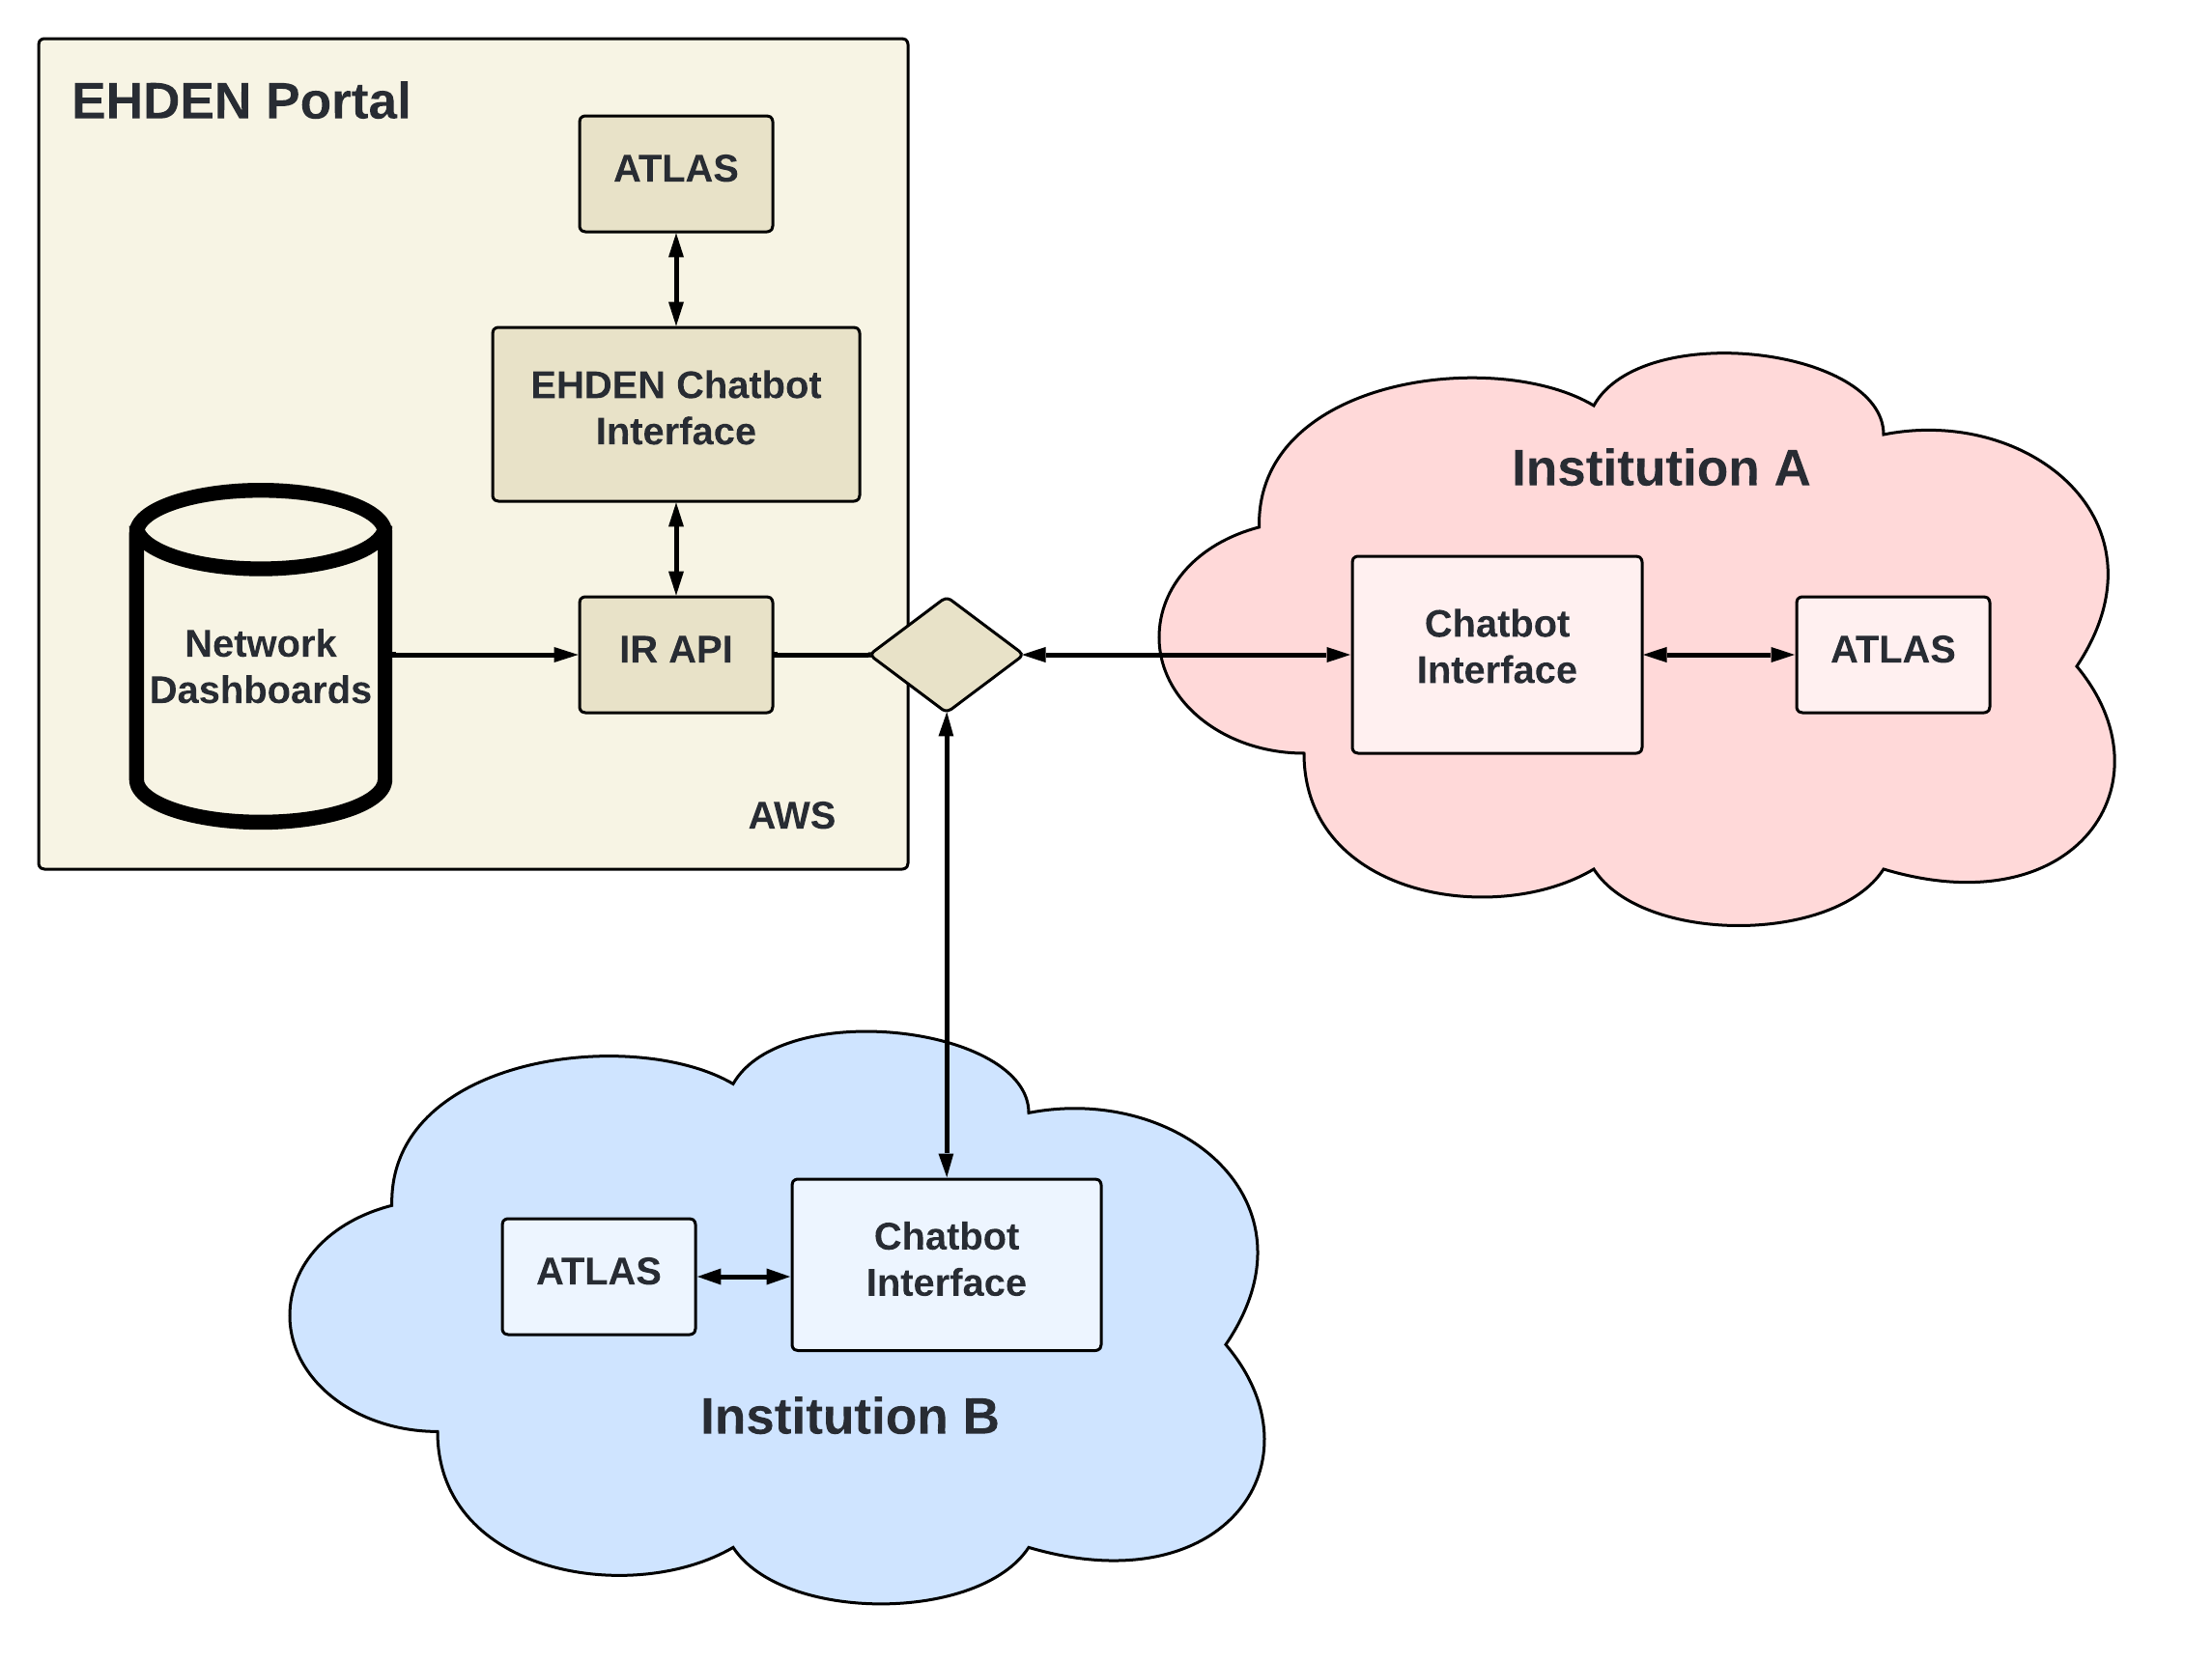
\includegraphics[width=0.9\textwidth]{figs/chapter4/network_diagram.png}
  \centering
  \caption{Network diagram illustrating the connections between the system and other institutions.}
  \label{fig_network}
\end{figure}

The {\ehden} Portal serves as the central hub, hosting the {\ehden} Chatbot Interface. Within this portal, the Network Dashboards provide metadata about various databases, which are crucial for the initial indexing and subsequent query building.

The {\ehden} Chatbot Interface interacts directly with the user, guiding them through the process of defining concept sets and cohorts. It communicates with the IR API to retrieve relevant questions and forms, which are then presented to the user for completion.

The {\ir} API acts as a mediator between the user inputs received via the Chatbot Interface and the ATLAS platform. It processes user queries, retrieves relevant database metadata, and prepares the necessary JSON structures for Cohort and Concept Set definitions.

Multiple institutions interact with the {\ehden} Portal {\ir} API, each with its own Chatbot Interface connected to its ATLAS instance. Institution A and Institution B represent different organizational units that utilize the {\ehden} infrastructure for their research needs. The institutions' Chatbot Interfaces communicate with their respective ATLAS instances and the {\ehden} Portal, ensuring data consistency and integration.

Institutions A and B, through their Chatbot Interfaces, interact with the {\ir} API and ATLAS to perform similar tasks. Each institution can define its cohorts and concept sets, leveraging the centralized capabilities of the {\ehden} infrastructure while maintaining individual ATLAS instances for specific research activities.
